% MCM/ICM 2026 LaTeX 主控文件 - Problem E (Sustainability)
% 编译方式:XeLaTeX + Biber(推荐用latexmk自动编译)
% !TEX program = xelatex
% !BIB program = biber

\documentclass{mcmthesis}

% 兼容性补丁:避免旧aux残留的chapter计数器导致hyperref报错
\newcounter{chapter}
\renewcommand{\thechapter}{\arabic{chapter}}

% MCM题目配置(比赛时务必修改tcn为真实队号)
\mcmsetup{
    tcn = {2617892},
    problem = {E},
    sheet = true,
    titleinsheet = true,
    keywordsinsheet = true,
    titlepage = false
}

% 目录开关
\makeatletter
\@ifundefined{showtoctrue}{}{\showtoctrue}
\makeatother

%=== 宏包加载 ===

% 字体与排版
\usepackage{palatino}
\usepackage{microtype}
\setlength{\emergencystretch}{2em}

% 页面与布局
\usepackage{lastpage}
\usepackage{zref-abspage}
\usepackage{float}
\usepackage{geometry}
\setlength{\headheight}{15pt}

% 数学公式
\usepackage{amsmath, amssymb, amsthm}
\usepackage{mathtools}

% 表格美化
\usepackage{booktabs}
\usepackage{tabularx}
\usepackage{longtable}
\usepackage{multirow}
\usepackage{array}

% 算法伪代码(顶会风格)
\usepackage[ruled, vlined, linesnumbered]{algorithm2e}
\SetAlgorithmName{Algorithm}{algorithm}{List of Algorithms}
\SetKwInput{KwIn}{Input}
\SetKwInput{KwOut}{Output}
\SetKwInput{KwData}{Data}
\SetKwInput{KwResult}{Result}

% 代码高亮
\usepackage{listings}
\lstset{
    basicstyle=\small\ttfamily,
    keywordstyle=\color{blue},
    commentstyle=\color{gray},
    numbers=left,
    numberstyle=\tiny\color{gray},
    frame=single,
    breaklines=true,
    tabsize=4
}

% 图形与颜色
\usepackage{graphicx}
\usepackage{subcaption}
\usepackage{xcolor}
\usepackage{tikz}
\usetikzlibrary{shapes, arrows, positioning, calc, fit, backgrounds}

% 列表与枚举
\usepackage{enumitem}
\setlist[enumerate]{itemsep=0pt, parsep=0pt}

% 超链接(最后加载)
\usepackage{hyperref}
\hypersetup{
    colorlinks=true,
    linkcolor=black,
    citecolor=green!50!black,
    urlcolor=blue!80!black
}

% 目录格式调整(紧凑行距)
\usepackage{tocloft}
\setlength{\cftbeforesecskip}{2pt}
\setlength{\cftbeforesubsecskip}{1pt}

% 参考文献
\usepackage[backend=biber, style=ieee, sorting=none]{biblatex}
\addbibresource{ref.bib}

%=== 自定义命令 ===

% 正文页数计数器(实现 Page X of Y)
\newcounter{mainpages}
\makeatletter
\newcommand{\savemainpages}{%
    \immediate\write\@auxout{\string\setcounter{mainpages}{\the\value{page}}}%
}
\makeatother

% 快捷引用命令
\newcommand{\figref}[1]{Fig.~\ref{#1}}
\newcommand{\tabref}[1]{Table~\ref{#1}}
\newcommand{\eqnref}[1]{Eq.~(\ref{#1})}
\newcommand{\algref}[1]{Algorithm~\ref{#1}}
\newcommand{\secref}[1]{Section~\ref{#1}}

% TODO标记命令(用于标识待填内容)
\newcommand{\TODO}[1]{\textcolor{red}{\textbf{[TODO: #1]}}}

%=== 文档元信息 ===

\title{A Sustainability-Oriented Multi-Criteria Decision Framework for \\
       \TODO{Problem E Topic: e.g., Ecosystem Restoration / Clean Energy Transition}}
\author{Team \#2617892}

%=== 正文开始 ===
\begin{document}

% Summary Sheet(摘要页,不计入页数)
\pagenumbering{arabic}
\setcounter{page}{0}
\pagestyle{empty}
\begin{abstract}%以下是25年C题的参考Abstract
    
To ensure a systematic and multidimensional approach to Olympic medal prediction, this study constructs a dynamic and coupled comprehensive \textbf{Predictive Framework}. This framework integrates various objectives, including medal distribution prediction, breakthrough country identification, event performance evaluation, and the impact analysis of coaching resource allocation. By employing multi-source heterogeneous data fusion and machine learning integration methods, we achieve an in-depth analysis and reliable prediction of the development patterns in competitive sports.

First, we develop a multidimensional predictive model to analyze Olympic medal patterns. Utilizing \textbf{Principal Component Analysis (PCA)} for dimensionality reduction and noise filtering of the Olympic event dataset, we combine \textbf{Long Short-Term Memory (LSTM)} networks to mine temporal features and integrate home advantage effects. A dual-channel \textbf{XGBoost-Bootstrap} model is established to generate predictions with a 95\% confidence interval. The results indicate an upward trend for countries such as the United States and the United Kingdom, while countries like France and China show a decline. The model exhibites a high accuracy with a low \textbf{MAE} and \textbf{MAPE}, demonstrating strong robustness. Through non-parametric testing, potential breakthrough countries are identified, with San Marino and Kuwait showing gold medal breakthrough probabilities of \textbf{84.7\%} and \textbf{68.4\%}, respectively.

Subsequently, we develop a \textbf{Difference-in-Differences (DID)} model to quantify the competitive benefits of coaching replacement and conduct statistical significance tests as well as parallel trends tests to ensure the reliability of our results. It is found that during the 2020-2024 period, Australia, South Korea, and Poland experienced significant "great coach" policy effects through strategic restructuring of their coaching teams. Based on this, we recommend prioritizing investment in high-elasticity projects. \textbf{SHapley Additive exPlanations (SHAP)} is further utilized to quantify event contributions, revealing that swimming and athletics serve as core contributing events to medal augmentation.

Furthermore, we explore the potential of a country to win its first-ever medal by constructing a \textbf{Hurdle-Tobit} fusion model. This model addresses the zero-inflation characteristics and heterogeneity between countries. The prediction results show that countries like Angola and Bangladesh have a probability of winning their first medal exceeding \textbf{45\%} in the next Games. Finally, we propose a strategic resource allocation plan using \textbf{Multiobjective Optimization} to balance the "depth" and "breadth" of National Olympic Committees (NOCs), suggesting that high-potential NOCs should prioritize multinational coach introductions in wrestling and table tennis.

In conclusion, our integrated framework synthesizes all models and analyses to present new insights and corresponding decision supports for the global sports community.

\begin{keywords}
    Olympic Medal Prediction, PCA-LSTM, XGBoost, DID Model, Hurdle-Tobit, SHAP Analysis.
\end{keywords}

\end{abstract}

\maketitle
\thispagestyle{empty}

% Contents(目录页,从第1页开始但不显示页码)
\newpage
\setcounter{page}{1}
\pagestyle{empty}
\tableofcontents
\thispagestyle{empty}

% 正文开始(从第3页开始显示页眉页码)
\newpage
\setcounter{page}{3}
\pagestyle{fancy}
\fancyhf{}
\fancyhead[L]{\small Team \#2617892}
\fancyhead[R]{\small Page \thepage\ of \themainpages}
\fancyfoot[C]{}

%=== Part I: Problem Understanding & System Definition ===

% Section 1: Introduction (问题重构与利益相关者)
% Section 1: Introduction
% 引言:问题背景 + 问题重述 + 利益相关者 + 本文工作

\section{Introduction}
\label{sec:intro}

%=== 1.1 问题背景:强调可持续性挑战 ===
\subsection{Problem Background}
\label{subsec:background}

% 【写作指导】E题引言需强调:
% 1. 环境问题的紧迫性与全球性
% 2. 多利益相关者的复杂博弈
% 3. 可持续发展的长期视角

The 21st century confronts humanity with unprecedented environmental challenges that demand integrated, systems-oriented solutions. \TODO{Describe the specific environmental context of Problem E, e.g., ecosystem degradation, climate adaptation, resource scarcity, clean energy transition.}

The complexity of this challenge arises from several intertwined factors:

\begin{itemize}[itemsep=0.3em]
    \item \textbf{Interconnected Systems:} Environmental, economic, and social systems are deeply coupled, with interventions in one domain producing cascading effects across others.
    
    \item \textbf{Temporal Dynamics:} Sustainability outcomes unfold over decades, requiring models that capture both short-term trade-offs and long-term equilibria.
    
    \item \textbf{Stakeholder Heterogeneity:} Different actors---governments, industries, communities, and future generations---hold divergent values and objectives that must be reconciled.
    
    \item \textbf{Deep Uncertainty:} Climate variability, technological disruptions, and policy shifts introduce substantial uncertainty into any planning framework.
\end{itemize}

\TODO{Add 1-2 paragraphs with specific statistics and references relevant to the Problem E topic. Cite authoritative sources such as IPCC, UN SDGs, or peer-reviewed literature.}

%=== 1.2 问题重述:精确界定任务 ===
\subsection{Restatement of the Problem}
\label{subsec:restatement}

To address the requirements of the 2026 ICM Problem E, we are tasked with developing a comprehensive analytical framework to:

\begin{enumerate}[itemsep=0.4em]
    \item \textbf{Task 1: \TODO{First Sub-Problem}}
    
    \TODO{Restate the first specific question from Problem E. Example: ``Develop a sustainability indicator system that captures environmental, economic, and social dimensions of [topic].''}
    
    \item \textbf{Task 2: \TODO{Second Sub-Problem}}
    
    \TODO{Restate the second specific question. Example: ``Model the dynamic interactions between [key system components] over a [time horizon].''}
    
    \item \textbf{Task 3: \TODO{Third Sub-Problem}}
    
    \TODO{Restate the third specific question. Example: ``Evaluate alternative policy scenarios and identify optimal intervention strategies.''}
    
    \item \textbf{Task 4: \TODO{Fourth Sub-Problem / Policy Memo}}
    
    \TODO{Restate the policy communication requirement. Example: ``Prepare a concise policy brief for [target decision-maker] summarizing key findings and recommendations.''}
\end{enumerate}

%=== 1.3 利益相关者与目标分析 ===
\subsection{Stakeholders and Objectives}
\label{subsec:stakeholders}

% 【E题核心】利益相关者分析是O奖论文的标志性要素
A sustainability-oriented decision framework must explicitly acknowledge the diverse stakeholders affected by and influencing the system. Table~\ref{tab:stakeholders} maps key stakeholders to their primary objectives and potential conflicts.

\begin{table}[H]
    \centering
    \caption{Stakeholder Analysis Matrix}
    \label{tab:stakeholders}
    \begin{tabularx}{\textwidth}{l X X X}
        \toprule
        \textbf{Stakeholder} & \textbf{Primary Objectives} & \textbf{Constraints} & \textbf{Potential Conflicts} \\
        \midrule
        \TODO{Government} & 
        \TODO{Environmental protection, economic growth, public welfare} & 
        \TODO{Budget limitations, political cycles} & 
        \TODO{Short-term growth vs. long-term sustainability} \\
        \addlinespace[0.5em]
        
        \TODO{Communities} & 
        \TODO{Livelihoods, health, cultural preservation} & 
        \TODO{Limited resources, information asymmetry} & 
        \TODO{Development vs. conservation} \\
        \addlinespace[0.5em]
        
        \TODO{Private Sector} & 
        \TODO{Profitability, market share, compliance} & 
        \TODO{Competition, capital constraints} & 
        \TODO{Cost externalization vs. responsibility} \\
        \addlinespace[0.5em]
        
        \TODO{NGOs} & 
        \TODO{Advocacy, transparency, equity} & 
        \TODO{Funding, influence} & 
        \TODO{Radical vs. incremental change} \\
        \addlinespace[0.5em]
        
        \TODO{Future Gen.} & 
        \TODO{Intergenerational equity, resources} & 
        \TODO{No direct voice} & 
        \TODO{Present vs. future well-being} \\
        \bottomrule
    \end{tabularx}
\end{table}

% 目标层次结构
Our framework adopts a \textbf{hierarchical objective structure} aligned with the three pillars of sustainability:

\begin{enumerate}[itemsep=0.2em]
    \item \textbf{Environmental Pillar:} \TODO{e.g., Minimize carbon emissions, preserve biodiversity, maintain ecosystem services}
    \item \textbf{Economic Pillar:} \TODO{e.g., Maximize cost-effectiveness, ensure economic viability, create green jobs}
    \item \textbf{Social Pillar:} \TODO{e.g., Promote equitable distribution, protect vulnerable populations, enhance quality of life}
\end{enumerate}

%=== 1.4 本文工作概述 ===
\subsection{Our Work}
\label{subsec:ourwork}

Our study introduces a \textbf{sustainability-oriented decision support framework} with the following methodological contributions:

\begin{enumerate}[itemsep=0.4em]
    \item \textbf{Three-Pillar Indicator System:}
    A comprehensive sustainability assessment framework integrating environmental, economic, and social dimensions through AHP-Entropy hybrid weighting.
    
    \item \textbf{System Dynamics Modeling:}
    A feedback-driven model capturing nonlinear interactions, tipping points, and long-term system trajectories under different policy regimes.
    
    \item \textbf{Scenario-Based Analysis:}
    Four carefully designed scenarios (BAU, Moderate, Aggressive, Stress Test) that span the policy option space and stress-test system resilience.
    
    \item \textbf{Multi-Criteria Decision Analysis:}
    TOPSIS-based ranking complemented by explicit trade-off frontier visualization to support transparent decision-making.
    
    \item \textbf{Actionable Policy Recommendations:}
    Tiered, stakeholder-specific recommendations with implementation roadmaps and adaptive management provisions.
\end{enumerate}

% 【插入框架流程图占位符】
\begin{figure}[H]
    \centering
    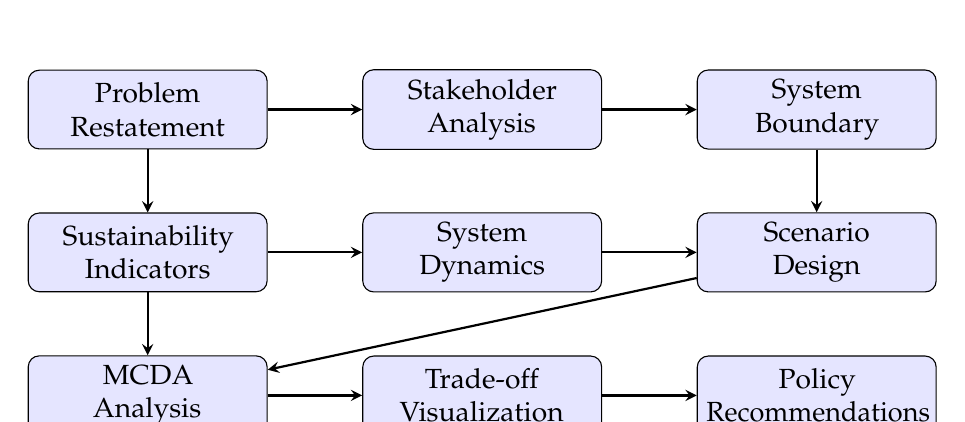
\begin{tikzpicture}[
        node distance=0.8cm and 1.2cm,
        block/.style={rectangle, draw, fill=blue!10, text width=2.8cm, minimum height=1cm, align=center, rounded corners},
        arrow/.style={->, >=stealth, thick}
    ]
        % 第一行:问题理解
        \node[block] (problem) {Problem\\Restatement};
        \node[block, right=of problem] (stakeholder) {Stakeholder\\Analysis};
        \node[block, right=of stakeholder] (boundary) {System\\Boundary};
        
        % 第二行:评估框架
        \node[block, below=of problem] (indicators) {Sustainability\\Indicators};
        \node[block, right=of indicators] (sd) {System\\Dynamics};
        \node[block, right=of sd] (scenarios) {Scenario\\Design};
        
        % 第三行:决策支持
        \node[block, below=of indicators] (mcda) {MCDA\\Analysis};
        \node[block, right=of mcda] (tradeoff) {Trade-off\\Visualization};
        \node[block, right=of tradeoff] (policy) {Policy\\Recommendations};
        
        % 连接箭头
        \draw[arrow] (problem) -- (stakeholder);
        \draw[arrow] (stakeholder) -- (boundary);
        \draw[arrow] (boundary) -- (scenarios);
        \draw[arrow] (problem) -- (indicators);
        \draw[arrow] (indicators) -- (sd);
        \draw[arrow] (sd) -- (scenarios);
        \draw[arrow] (indicators) -- (mcda);
        \draw[arrow] (scenarios) -- (mcda);
        \draw[arrow] (mcda) -- (tradeoff);
        \draw[arrow] (tradeoff) -- (policy);
    \end{tikzpicture}
    \caption{Overview of our sustainability-oriented decision framework.}
    \label{fig:framework}
\end{figure}


% Section 2: Assumptions and System Boundary (假设与系统边界)
% Section 2: Assumptions and Justifications
% 假设条件及其合理性说明

\section{Assumptions and Justifications}
\label{sec:assumptions}

To establish a reasonable and solvable mathematical model, we make the following assumptions. Each assumption is justified with a brief rationale.

\begin{enumerate}[label=\textbf{H\arabic*.}, leftmargin=2em, itemsep=0.6em]
    
    \item \textbf{Data Integrity Assumption.}
    The provided dataset is complete and representative of the real-world scenario.
    
    \textit{Justification:} The official dataset from COMAP is assumed to undergo quality control. Missing values, if any, are handled in our preprocessing pipeline.
    
    \item \textbf{Temporal Stability Assumption.}
    The underlying patterns and trends observed in historical data remain consistent during the prediction horizon.
    
    \textit{Justification:} Short-term forecasting (e.g., 1--2 Olympic cycles) typically does not experience drastic structural changes unless major disruptions occur.
    
    \item \textbf{Independence Assumption.}
    The observations are independently and identically distributed (i.i.d.) within each time window.
    
    \textit{Justification:} This is a standard assumption for many statistical and machine learning models, enabling the use of classical estimators.
    
    \item \textbf{Policy Lag Assumption.}
    There exists a time delay between policy implementation and observable effects.
    
    \textit{Justification:} Government policies typically require administrative processes, public communication, and behavioral adaptation periods before measurable impacts emerge.
    
    \item \textbf{External Shock Exclusion.}
    We assume no major external shocks (e.g., pandemics, wars, natural disasters) occur during the modeling period.
    
    \textit{Justification:} Such events are inherently unpredictable and would require scenario-based analysis beyond the scope of this competition.

\end{enumerate}


% Section 3: Notations (符号说明)
% Section 3: Notations
% 符号说明表:按类别组织,适应E题可持续性建模

\section{Notations}
\label{sec:notations}

For clarity and consistency throughout this paper, we summarize the key symbols used in our sustainability assessment framework in Table~\ref{tab:notations}.

\begin{table}[H]
    \centering
    \caption{Summary of Key Notations}
    \label{tab:notations}
    \begin{tabularx}{\textwidth}{c X c}
        \toprule
        \textbf{Symbol} & \textbf{Description} & \textbf{Unit} \\
        \midrule
        \multicolumn{3}{l}{\textit{\textbf{Index Sets}}} \\
        $t$ & Time period index, $t \in \mathcal{T} = \{1, 2, \ldots, T\}$ & year \\
        $i$ & Indicator index, $i \in \mathcal{I} = \{1, 2, \ldots, n\}$ & -- \\
        $s$ & Scenario index, $s \in \mathcal{S} = \{\text{BAU}, \text{MOD}, \text{AGG}, \text{STRESS}\}$ & -- \\
        $k$ & Stakeholder index, $k \in \mathcal{K}$ & -- \\
        \midrule
        \multicolumn{3}{l}{\textit{\textbf{Sustainability Indicators (Three Pillars)}}} \\
        $E_i$ & $i$-th environmental indicator value & varies \\
        $C_j$ & $j$-th economic indicator value & varies \\
        $S_l$ & $l$-th social indicator value & varies \\
        $\mathbf{X}$ & Aggregated indicator matrix, $\mathbf{X} \in \mathbb{R}^{n \times T}$ & -- \\
        \midrule
        \multicolumn{3}{l}{\textit{\textbf{Weighting and Aggregation}}} \\
        $w_i$ & Weight assigned to indicator $i$, $\sum_i w_i = 1$ & -- \\
        $w_i^{\text{AHP}}$ & AHP-derived subjective weight & -- \\
        $w_i^{\text{Ent}}$ & Entropy-derived objective weight & -- \\
        $\lambda$ & Combination coefficient for hybrid weighting, $\lambda \in [0,1]$ & -- \\
        $U$ & Composite sustainability score, $U = \sum_i w_i \cdot \tilde{X}_i$ & -- \\
        \midrule
        \multicolumn{3}{l}{\textit{\textbf{System Dynamics Variables}}} \\
        $\mathbf{S}(t)$ & Stock variables vector at time $t$ (e.g., resource stock, capital) & varies \\
        $\mathbf{F}(t)$ & Flow variables vector at time $t$ (e.g., emissions rate, investment) & varies/yr \\
        $\tau$ & Time delay parameter for feedback loops & year \\
        $\kappa$ & Carrying capacity or system limit & varies \\
        \midrule
        \multicolumn{3}{l}{\textit{\textbf{Scenario Parameters}}} \\
        $\pi_s$ & Policy intensity under scenario $s$ & \% or \$ \\
        $\Delta_s(t)$ & Scenario-specific intervention magnitude at time $t$ & varies \\
        $P_{\text{shock}}$ & Probability of extreme event (stress scenario) & -- \\
        \midrule
        \multicolumn{3}{l}{\textit{\textbf{Multi-Criteria Decision Analysis (MCDA)}}} \\
        $\mathbf{D}$ & Decision matrix, $\mathbf{D} \in \mathbb{R}^{m \times n}$ (alternatives $\times$ criteria) & -- \\
        $A^+, A^-$ & Ideal and anti-ideal solutions in TOPSIS & -- \\
        $d_j^+, d_j^-$ & Distance to ideal/anti-ideal for alternative $j$ & -- \\
        $C_j^*$ & Relative closeness coefficient for alternative $j$ & -- \\
        \midrule
        \multicolumn{3}{l}{\textit{\textbf{Economic Parameters}}} \\
        $r$ & Social discount rate & \%/yr \\
        $\text{NPV}$ & Net Present Value of intervention & \$ \\
        $B/C$ & Benefit-Cost Ratio & -- \\
        $\text{ROI}$ & Return on Investment for sustainability intervention & \% \\
        \midrule
        \multicolumn{3}{l}{\textit{\textbf{Sensitivity Analysis}}} \\
        $\theta$ & Generic parameter subject to perturbation & varies \\
        $\Delta \theta$ & Perturbation magnitude for sensitivity analysis & \% \\
        $\eta_{\theta}$ & Sensitivity elasticity: $\eta = \frac{\partial U / U}{\partial \theta / \theta}$ & -- \\
        \bottomrule
    \end{tabularx}
\end{table}

% 补充说明
\noindent\textbf{Normalization Convention.} Unless otherwise stated, all indicators are normalized to $[0, 1]$ using min-max scaling:
\begin{equation}
    \tilde{X}_i = \frac{X_i - X_i^{\min}}{X_i^{\max} - X_i^{\min}}
    \label{eq:normalization}
\end{equation}
For ``negative'' indicators (where lower is better, e.g., pollution), we apply reverse scaling: $\tilde{X}_i = 1 - \frac{X_i - X_i^{\min}}{X_i^{\max} - X_i^{\min}}$.


%=== Part II: Sustainability Assessment Framework ===

% Section 4: Sustainability Indicator System (可持续性指标体系)
% Section 4: Sustainability Indicator System
% 可持续性指标体系:环境-经济-社会三支柱框架

\section{Sustainability Indicator System}
\label{sec:indicators}

% 【E题核心建模组件】本节是O奖论文的标志性章节

%=== 4.1 指标体系设计原则 ===
\subsection{Design Principles}
\label{subsec:indicator_principles}

Our sustainability indicator system adheres to the following design principles, ensuring scientific rigor and practical relevance:

\begin{enumerate}[itemsep=0.3em]
    \item \textbf{Three-Pillar Coverage:} Indicators span environmental, economic, and social dimensions in alignment with the UN Sustainable Development Goals (SDGs) framework.
    
    \item \textbf{SMART Criteria:} Each indicator is \textbf{S}pecific, \textbf{M}easurable, \textbf{A}chievable, \textbf{R}elevant, and \textbf{T}ime-bound.
    
    \item \textbf{Data Availability:} Prioritize indicators with reliable, publicly accessible data sources to ensure reproducibility.
    
    \item \textbf{Sensitivity:} Indicators should be responsive to policy interventions within the modeling horizon.
    
    \item \textbf{Independence:} Minimize redundancy by selecting indicators that capture distinct aspects of sustainability.
\end{enumerate}

%=== 4.2 三支柱指标体系 ===
\subsection{Three-Pillar Indicator Framework}
\label{subsec:three_pillars}

Table~\ref{tab:indicators} presents our hierarchical indicator system organized by pillar, sub-category, and specific metrics.

\begin{table}[H]
    \centering
    \caption{Hierarchical Sustainability Indicator Framework}
    \label{tab:indicators}
    \begin{tabularx}{\textwidth}{l l X c c}
        \toprule
        \textbf{Pillar} & \textbf{Sub-Category} & \textbf{Indicator} & \textbf{Direction} & \textbf{Weight} \\
        \midrule
        \multirow{6}{*}{\rotatebox{90}{\textbf{Environmental}}} 
        & Climate & \TODO{e.g., GHG Emissions (tCO$_2$eq)} & $\downarrow$ & \TODO{$w_1$} \\
        & Climate & \TODO{e.g., Renewable Energy Share (\%)} & $\uparrow$ & \TODO{$w_2$} \\
        & Resources & \TODO{e.g., Water Use Efficiency (m$^3$/\$)} & $\uparrow$ & \TODO{$w_3$} \\
        & Resources & \TODO{e.g., Material Circularity Rate (\%)} & $\uparrow$ & \TODO{$w_4$} \\
        & Ecosystem & \TODO{e.g., Biodiversity Index} & $\uparrow$ & \TODO{$w_5$} \\
        & Pollution & \TODO{e.g., Air Quality Index (PM2.5)} & $\downarrow$ & \TODO{$w_6$} \\
        \midrule
        \multirow{5}{*}{\rotatebox{90}{\textbf{Economic}}} 
        & Growth & \TODO{e.g., GDP per Capita (\$)} & $\uparrow$ & \TODO{$w_7$} \\
        & Employment & \TODO{e.g., Green Job Creation (jobs/yr)} & $\uparrow$ & \TODO{$w_8$} \\
        & Investment & \TODO{e.g., Sustainability Investment (\% GDP)} & $\uparrow$ & \TODO{$w_9$} \\
        & Efficiency & \TODO{e.g., Cost-Effectiveness Ratio} & $\uparrow$ & \TODO{$w_{10}$} \\
        & Risk & \TODO{e.g., Economic Vulnerability Index} & $\downarrow$ & \TODO{$w_{11}$} \\
        \midrule
        \multirow{5}{*}{\rotatebox{90}{\textbf{Social}}} 
        & Equity & \TODO{e.g., Gini Coefficient} & $\downarrow$ & \TODO{$w_{12}$} \\
        & Health & \TODO{e.g., Life Expectancy (years)} & $\uparrow$ & \TODO{$w_{13}$} \\
        & Education & \TODO{e.g., Education Access Index} & $\uparrow$ & \TODO{$w_{14}$} \\
        & Resilience & \TODO{e.g., Community Adaptive Capacity} & $\uparrow$ & \TODO{$w_{15}$} \\
        & Participation & \TODO{e.g., Public Engagement Rate (\%)} & $\uparrow$ & \TODO{$w_{16}$} \\
        \bottomrule
    \end{tabularx}
    \vspace{0.3em}
    \footnotesize{Note: $\uparrow$ indicates ``higher is better''; $\downarrow$ indicates ``lower is better''.}
\end{table}

%=== 4.3 指标权重确定:AHP-熵权法混合 ===
\subsection{Hybrid Weighting: AHP-Entropy Method}
\label{subsec:weighting}

We employ a hybrid weighting approach that combines \textbf{subjective expert judgment} (AHP) with \textbf{objective data-driven analysis} (Entropy Method) to ensure robustness and legitimacy.

\subsubsection{Analytic Hierarchy Process (AHP)}
The AHP derives weights through pairwise comparison of indicator importance by domain experts:

\begin{enumerate}[itemsep=0.2em]
    \item Construct pairwise comparison matrix $\mathbf{A} = [a_{ij}]$ where $a_{ij}$ represents the relative importance of indicator $i$ over $j$ on a 1--9 scale.
    \item Compute the principal eigenvector $\mathbf{w}^{\text{AHP}}$ satisfying $\mathbf{A} \mathbf{w}^{\text{AHP}} = \lambda_{\max} \mathbf{w}^{\text{AHP}}$.
    \item Verify consistency using the Consistency Ratio: $\text{CR} = \frac{\text{CI}}{\text{RI}} < 0.10$, where $\text{CI} = \frac{\lambda_{\max} - n}{n - 1}$.
\end{enumerate}

\subsubsection{Entropy Weighting Method}
The entropy method derives weights based on information content in the data:

\begin{equation}
    e_i = -\frac{1}{\ln m} \sum_{j=1}^{m} p_{ij} \ln p_{ij}, \quad w_i^{\text{Ent}} = \frac{1 - e_i}{\sum_{k}(1 - e_k)}
    \label{eq:entropy}
\end{equation}
where $p_{ij} = \tilde{X}_{ij} / \sum_j \tilde{X}_{ij}$ is the proportion of indicator $i$ for alternative $j$.

\subsubsection{Hybrid Combination}
The final weights combine both methods:
\begin{equation}
    w_i = \lambda \cdot w_i^{\text{AHP}} + (1 - \lambda) \cdot w_i^{\text{Ent}}, \quad \lambda \in [0, 1]
    \label{eq:hybrid_weight}
\end{equation}

We set $\lambda = 0.5$ as a balanced default; sensitivity to $\lambda$ is examined in Section~\ref{sec:sensitivity}.

%=== 4.4 复合可持续性得分计算 ===
\subsection{Composite Sustainability Score}
\label{subsec:composite_score}

The composite sustainability score for alternative $j$ at time $t$ is computed as:

\begin{equation}
    U_j(t) = \underbrace{\sum_{i \in \mathcal{E}} w_i \cdot \tilde{E}_{ij}(t)}_{\text{Environmental Score}} + \underbrace{\sum_{i \in \mathcal{C}} w_i \cdot \tilde{C}_{ij}(t)}_{\text{Economic Score}} + \underbrace{\sum_{i \in \mathcal{S}} w_i \cdot \tilde{S}_{ij}(t)}_{\text{Social Score}}
    \label{eq:composite}
\end{equation}

where $\tilde{E}$, $\tilde{C}$, $\tilde{S}$ are normalized indicator values within each pillar.

% 指标体系可视化占位符
\begin{figure}[H]
    \centering
    \fbox{\parbox[c][0.28\textheight][c]{0.9\textwidth}{
        \centering
        \textbf{Sustainability Indicator Hierarchy Diagram}
        \par\vspace{1em}
        \small \TODO{Replace with actual hierarchy diagram or radar chart showing the three pillars and their sub-indicators. Consider using a treemap, sunburst chart, or hierarchical tree structure.}
    }}
    \caption{Hierarchical structure of the three-pillar sustainability indicator system.}
    \label{fig:indicator_hierarchy}
\end{figure}


% Section 5: System Dynamics Model (系统动力学建模)
% Section 5: System Dynamics Model
% 系统动力学建模:捕捉非线性反馈与长期演化

\section{System Dynamics Model}
\label{sec:system_model}

% 【E题核心】系统动力学是O奖论文的标志性方法论

%=== 5.1 系统动力学方法论 ===
\subsection{System Dynamics Approach}
\label{subsec:sd_methodology}

System Dynamics (SD) is a methodology for studying complex systems characterized by:
\begin{itemize}[itemsep=0.2em]
    \item \textbf{Feedback Loops:} Circular causality where effects become causes, creating reinforcing ($+$) or balancing ($-$) dynamics.
    \item \textbf{Stock-Flow Structure:} Accumulations (stocks) change through inflows and outflows.
    \item \textbf{Time Delays:} Lags between cause and effect that can destabilize systems.
    \item \textbf{Nonlinearity:} Relationships that change in magnitude or direction across operating ranges.
\end{itemize}

SD is particularly suited for sustainability problems because it captures the long-term, interconnected nature of environmental-economic-social systems that linear optimization cannot adequately represent~\cite{sterman2000business, meadows2004limits}.

%=== 5.2 因果回路图 ===
\subsection{Causal Loop Diagram}
\label{subsec:cld}

Figure~\ref{fig:cld} presents the high-level causal loop diagram (CLD) capturing key feedback mechanisms in our system.

\begin{figure}[H]
    \centering
    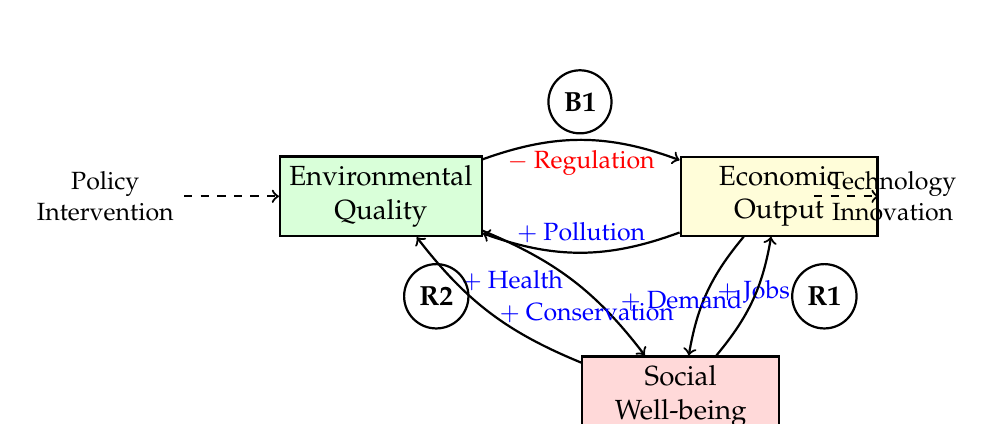
\begin{tikzpicture}[
        node distance=2.5cm,
        stock/.style={rectangle, draw, thick, minimum width=2.5cm, minimum height=1cm, align=center},
        arrow/.style={->, thick},
        plus/.style={font=\small, blue},
        minus/.style={font=\small, red}
    ]
        % 核心存量
        \node[stock, fill=green!15] (env) {Environmental\\Quality};
        \node[stock, fill=yellow!15, right=of env] (econ) {Economic\\Output};
        \node[stock, fill=red!15, below right=1.5cm and 1.25cm of env] (social) {Social\\Well-being};
        
        % 反馈回路1:经济-环境权衡 (Balancing)
        \draw[arrow] (econ) to[bend left=20] node[above, plus] {$+$ Pollution} (env);
        \draw[arrow] (env) to[bend left=20] node[below, minus] {$-$ Regulation} (econ);
        \node[draw, circle, thick] at ($(env)!0.5!(econ) + (0, 1.2)$) {\textbf{B1}};
        
        % 反馈回路2:经济-社会正反馈 (Reinforcing)
        \draw[arrow] (econ) to[bend right=15] node[right, plus] {$+$ Jobs} (social);
        \draw[arrow] (social) to[bend right=15] node[left, plus] {$+$ Demand} (econ);
        \node[draw, circle, thick] at ($(econ)!0.5!(social) + (1.2, 0)$) {\textbf{R1}};
        
        % 反馈回路3:环境-社会 (Reinforcing)
        \draw[arrow] (env) to[bend left=15] node[left, plus] {$+$ Health} (social);
        \draw[arrow] (social) to[bend left=15] node[right, plus] {$+$ Conservation} (env);
        \node[draw, circle, thick] at ($(env)!0.5!(social) + (-1.2, 0)$) {\textbf{R2}};
        
        % 外生输入
        \node[align=center, font=\small] at (-3.5, 0) {Policy\\Intervention};
        \draw[->, dashed, thick] (-2.5, 0) -- (env);
        
        \node[align=center, font=\small] at (6.5, 0) {Technology\\Innovation};
        \draw[->, dashed, thick] (5.5, 0) -- (econ);
    \end{tikzpicture}
    \caption{Causal Loop Diagram showing key feedback structures. \textbf{R1, R2}: Reinforcing loops; \textbf{B1}: Balancing loop.}
    \label{fig:cld}
\end{figure}

\noindent\textbf{Key Feedback Loops:}
\begin{itemize}[itemsep=0.3em]
    \item \textbf{B1 (Economic-Environmental Balancing):} Economic growth increases pollution, which triggers environmental degradation and regulatory responses that constrain growth---a classic ``limits to growth'' dynamic.
    
    \item \textbf{R1 (Economic-Social Reinforcing):} Economic output creates jobs and income, enhancing social well-being, which in turn supports consumer demand and economic growth.
    
    \item \textbf{R2 (Environmental-Social Reinforcing):} Environmental quality improves public health and quality of life, which increases public support for conservation, further enhancing environmental quality.
\end{itemize}

%=== 5.3 存量-流量结构 ===
\subsection{Stock-Flow Structure}
\label{subsec:stock_flow}

The SD model is formalized through differential equations describing stock accumulation:

\subsubsection{Environmental Subsystem}
\begin{equation}
    \frac{d E_{\text{stock}}(t)}{dt} = R_{\text{regen}}(t) - D_{\text{depletion}}(t) - P_{\text{pollution}}(t) + I_{\text{restoration}}(t)
    \label{eq:env_stock}
\end{equation}
where:
\begin{itemize}[itemsep=0.1em]
    \item $E_{\text{stock}}$: Environmental resource stock (e.g., forest cover, fish population, air quality)
    \item $R_{\text{regen}}$: Natural regeneration rate
    \item $D_{\text{depletion}}$: Resource extraction/depletion rate
    \item $P_{\text{pollution}}$: Pollution accumulation
    \item $I_{\text{restoration}}$: Policy-driven restoration investment
\end{itemize}

\subsubsection{Economic Subsystem}
\begin{equation}
    \frac{d K(t)}{dt} = I(t) - \delta K(t), \quad Y(t) = A(t) \cdot K(t)^{\alpha} \cdot L(t)^{1-\alpha} \cdot E_{\text{stock}}(t)^{\gamma}
    \label{eq:econ_stock}
\end{equation}
where $K$ is capital stock, $I$ is investment, $\delta$ is depreciation, and $Y$ is output following an extended Cobb-Douglas production function with environmental factor $E_{\text{stock}}^{\gamma}$.

\subsubsection{Social Subsystem}
\begin{equation}
    \frac{d W(t)}{dt} = \beta_1 \cdot \ln(Y(t)/L(t)) + \beta_2 \cdot E_{\text{stock}}(t) - \beta_3 \cdot \text{Inequality}(t)
    \label{eq:social_stock}
\end{equation}
where $W$ represents aggregate social well-being as a function of income, environmental quality, and inequality.

%=== 5.4 关键参数与校准 ===
\subsection{Key Parameters and Calibration}
\label{subsec:sd_calibration}

\begin{table}[H]
    \centering
    \caption{System Dynamics Model Parameters}
    \label{tab:sd_params}
    \begin{tabularx}{\textwidth}{l X c c}
        \toprule
        \textbf{Parameter} & \textbf{Description} & \textbf{Value} & \textbf{Source} \\
        \midrule
        $R_{\text{regen}}$ & Natural regeneration rate & \TODO{value} & \TODO{source} \\
        $\delta$ & Capital depreciation rate & \TODO{value} & \TODO{source} \\
        $\alpha$ & Capital share in production & \TODO{value} & \TODO{source} \\
        $\gamma$ & Environmental elasticity of output & \TODO{value} & \TODO{source} \\
        $\tau_{\text{delay}}$ & Policy implementation delay & \TODO{value} & \TODO{source} \\
        $\kappa$ & Environmental carrying capacity & \TODO{value} & \TODO{source} \\
        \bottomrule
    \end{tabularx}
\end{table}

%=== 5.5 临界点与杠杆点识别 ===
\subsection{Tipping Points and Leverage Points}
\label{subsec:tipping_points}

A key insight from SD analysis is the identification of:

\begin{itemize}[itemsep=0.3em]
    \item \textbf{Tipping Points:} Thresholds beyond which system behavior changes qualitatively (e.g., ecosystem collapse, runaway climate feedback).
    
    \item \textbf{Leverage Points:} Places in the system where small interventions can produce large, lasting changes~\cite{meadows1999leverage}.
\end{itemize}

\TODO{Based on model simulation, identify specific tipping points (e.g., ``When environmental stock falls below X\% of carrying capacity, regeneration collapses'') and leverage points (e.g., ``Increasing restoration investment efficiency by 10\% has 3x the impact of equivalent pollution reduction'').}

% SD模型输出占位符
\begin{figure}[H]
    \centering
    \fbox{\parbox[c][0.25\textheight][c]{0.9\textwidth}{
        \centering
        \textbf{System Dynamics Simulation Output}
        \par\vspace{1em}
        \small \TODO{Replace with time-series plots showing the evolution of key stocks (Environmental Quality, Economic Output, Social Well-being) under baseline conditions. Include identification of tipping points and leverage points.}
    }}
    \caption{Baseline System Dynamics simulation results showing stock trajectories over time.}
    \label{fig:sd_baseline}
\end{figure}


%=== Part III: Scenario Analysis & Decision Support ===

% Section 6: Scenario Design and Simulation (情景设计与模拟)
% Section 6: Scenario Design and Simulation
% 情景设计与模拟:E题核心分析框架

\section{Scenario Design and Simulation}
\label{sec:scenarios}

% 【E题核心】情景分析是O奖论文的必备组件

%=== 6.1 情景设计原则 ===
\subsection{Scenario Design Principles}
\label{subsec:scenario_principles}

Our scenario framework follows established best practices in sustainability assessment:

\begin{enumerate}[itemsep=0.3em]
    \item \textbf{Plausibility:} Each scenario is grounded in realistic policy options and technological trajectories.
    
    \item \textbf{Consistency:} Internal logic is maintained---policy choices align with socioeconomic assumptions.
    
    \item \textbf{Diversity:} Scenarios span the range of possible futures, from conservative to transformative.
    
    \item \textbf{Relevance:} Scenarios address the specific decision context of \TODO{target stakeholder/decision}.
    
    \item \textbf{Challenge:} At least one scenario stress-tests system resilience under extreme conditions.
\end{enumerate}

%=== 6.2 四大情景定义 ===
\subsection{Four Representative Scenarios}
\label{subsec:four_scenarios}

We design four scenarios that span the policy option space:

\begin{table}[H]
    \centering
    \caption{Summary of Scenario Specifications}
    \label{tab:scenarios}
    \begin{tabularx}{\textwidth}{l X X c}
        \toprule
        \textbf{Scenario} & \textbf{Policy Description} & \textbf{Key Parameters} & \textbf{Time Horizon} \\
        \midrule
        \textbf{S1: Business-as-Usual (BAU)} & 
        Continuation of current policies with no additional interventions. Baseline for comparison. & 
        \TODO{e.g., Current emission rates, existing regulations} & 
        \TODO{2025--2050} \\
        \addlinespace[0.5em]
        
        \textbf{S2: Moderate Intervention (MOD)} & 
        Incremental policy adjustments aligned with current pledges (e.g., NDCs, existing commitments). & 
        \TODO{e.g., 30\% emission reduction, moderate investment} & 
        \TODO{2025--2050} \\
        \addlinespace[0.5em]
        
        \textbf{S3: Aggressive Transition (AGG)} & 
        Transformative policy shift toward sustainability. Ambitious targets aligned with 1.5°C pathway or equivalent. & 
        \TODO{e.g., 70\% emission reduction, major investment} & 
        \TODO{2025--2050} \\
        \addlinespace[0.5em]
        
        \textbf{S4: Climate Shock (STRESS)} & 
        Stress test: Baseline policies plus an extreme climate event (e.g., drought, flood, pandemic) occurring at \TODO{year}. & 
        \TODO{e.g., 20\% productivity shock, emergency costs} & 
        \TODO{2025--2050} \\
        \bottomrule
    \end{tabularx}
\end{table}

%=== 6.3 情景参数化 ===
\subsection{Scenario Parameterization}
\label{subsec:scenario_params}

Each scenario modifies the System Dynamics model through specific parameter adjustments:

\subsubsection{Scenario S1: Business-as-Usual}
\begin{align}
    I_{\text{restoration}}(t) &= I_0 \quad \text{(constant at current level)} \label{eq:s1_invest} \\
    P_{\text{pollution}}(t) &= P_0 \cdot (1 + g_p)^t \quad \text{(growing at historical rate } g_p \text{)} \label{eq:s1_pollution}
\end{align}

\subsubsection{Scenario S2: Moderate Intervention}
% [TODO: Set r_mod and rho_mod values based on actual policy scenarios]
\begin{align}
    I_{\text{restoration}}(t) &= I_0 \cdot (1 + r_{\text{mod}})^t \quad \text{(moderate investment growth)} \label{eq:s2_invest} \\
    P_{\text{pollution}}(t) &= P_0 \cdot (1 - \rho_{\text{mod}})^t \quad \text{(gradual reduction)} \label{eq:s2_pollution}
\end{align}

\subsubsection{Scenario S3: Aggressive Transition}
% [TODO: Set r_agg and rho_agg values based on actual policy scenarios]
\begin{align}
    I_{\text{restoration}}(t) &= I_0 \cdot (1 + r_{\text{agg}})^t \quad \text{(ambitious investment growth)} \label{eq:s3_invest} \\
    P_{\text{pollution}}(t) &= P_0 \cdot \exp(-\rho_{\text{agg}} \cdot t) \quad \text{(exponential reduction)} \label{eq:s3_pollution}
\end{align}

\subsubsection{Scenario S4: Climate Shock}
% [TODO: Set sigma_shock and kappa_recovery values based on stress scenarios]
\begin{equation}
    Y(t) = Y_{\text{BAU}}(t) \cdot 
    \begin{cases}
        1 & \text{if } t < t_{\text{shock}} \\
        (1 - \sigma_{\text{shock}}) \cdot \exp(\kappa_{\text{recovery}} \cdot (t - t_{\text{shock}})) & \text{if } t \geq t_{\text{shock}}
    \end{cases}
    \label{eq:s4_shock}
\end{equation}

%=== 6.4 模拟结果 ===
\subsection{Simulation Results}
\label{subsec:simulation_results}

% 核心结果图表占位符
\begin{figure}[H]
    \centering
    \begin{subfigure}[t]{0.48\textwidth}
        \centering
        \fbox{\parbox[c][0.22\textheight][c]{\textwidth}{
            \centering
            \textbf{(a) Environmental Quality Trajectories}
            \par\vspace{0.5em}
            \small \TODO{Time-series plot showing $E_{\text{stock}}(t)$ for all four scenarios. Highlight tipping point if BAU crosses threshold.}
        }}
        \caption{Environmental stock under four scenarios}
        \label{fig:scenario_env}
    \end{subfigure}\hfill
    \begin{subfigure}[t]{0.48\textwidth}
        \centering
        \fbox{\parbox[c][0.22\textheight][c]{\textwidth}{
            \centering
            \textbf{(b) Economic Output Trajectories}
            \par\vspace{0.5em}
            \small \TODO{Time-series plot showing $Y(t)$ for all four scenarios. Show initial cost of AGG but long-term benefits.}
        }}
        \caption{Economic output under four scenarios}
        \label{fig:scenario_econ}
    \end{subfigure}
    
    \vspace{0.5cm}
    
    \begin{subfigure}[t]{0.48\textwidth}
        \centering
        \fbox{\parbox[c][0.22\textheight][c]{\textwidth}{
            \centering
            \textbf{(c) Social Well-being Trajectories}
            \par\vspace{0.5em}
            \small \TODO{Time-series plot showing $W(t)$ for all four scenarios.}
        }}
        \caption{Social well-being under four scenarios}
        \label{fig:scenario_social}
    \end{subfigure}\hfill
    \begin{subfigure}[t]{0.48\textwidth}
        \centering
        \fbox{\parbox[c][0.22\textheight][c]{\textwidth}{
            \centering
            \textbf{(d) Composite Sustainability Score}
            \par\vspace{0.5em}
            \small \TODO{Time-series plot showing $U(t)$ for all four scenarios.}
        }}
        \caption{Composite sustainability score}
        \label{fig:scenario_composite}
    \end{subfigure}
    \caption{System Dynamics simulation results across four scenarios (2025--2050).}
    \label{fig:scenario_results}
\end{figure}

%=== 6.5 关键发现 ===
\subsection{Key Findings}
\label{subsec:scenario_findings}

\TODO{Summarize the key insights from scenario comparison. Example structure:}

\begin{enumerate}[itemsep=0.4em]
    \item \textbf{BAU Unsustainability:} Under Business-as-Usual, environmental quality crosses the tipping point by \TODO{year}, triggering \TODO{consequence}.
    
    \item \textbf{Moderate vs. Aggressive Trade-offs:} MOD achieves \TODO{X\%} improvement in sustainability score but requires \TODO{Y\%} less investment than AGG. However, AGG avoids \TODO{specific risk}.
    
    \item \textbf{Shock Resilience:} The STRESS scenario reveals that systems under AGG recover \TODO{Z times faster} than under BAU, demonstrating the resilience value of sustainability investments.
    
    \item \textbf{Temporal Dynamics:} The ``green paradox'' is observed: AGG shows \TODO{short-term cost description} but yields net benefits by \TODO{breakeven year}.
\end{enumerate}


% Section 7: Multi-Criteria Decision Analysis (多准则决策分析)
% Section 7: Multi-Criteria Decision Analysis
% 多准则决策分析:TOPSIS与权衡可视化

\section{Multi-Criteria Decision Analysis}
\label{sec:mcda}

% 【E题核心】MCDA将技术分析转化为决策支持

%=== 7.1 MCDA方法论 ===
\subsection{MCDA Methodology}
\label{subsec:mcda_methodology}

Multi-Criteria Decision Analysis (MCDA) provides a structured framework for evaluating alternatives against multiple, potentially conflicting objectives~\cite{velasquez2013analysis}. For sustainability decisions involving environmental-economic-social trade-offs, MCDA offers:

\begin{itemize}[itemsep=0.2em]
    \item \textbf{Transparency:} Explicit articulation of criteria and weights.
    \item \textbf{Comprehensiveness:} Simultaneous consideration of all sustainability pillars.
    \item \textbf{Flexibility:} Accommodation of diverse stakeholder preferences through weight adjustment.
    \item \textbf{Defensibility:} Systematic documentation of decision logic.
\end{itemize}

We employ \textbf{TOPSIS} (Technique for Order Preference by Similarity to Ideal Solution) as our primary ranking method, complemented by trade-off frontier visualization.

%=== 7.2 决策矩阵构建 ===
\subsection{Decision Matrix Construction}
\label{subsec:decision_matrix}

The decision matrix $\mathbf{D}$ summarizes scenario performance across all indicators at the end of the projection horizon ($t = T$):

\begin{table}[H]
    \centering
    \caption{Decision Matrix: Scenario Performance on Sustainability Indicators}
    \label{tab:decision_matrix}
    \begin{tabular}{l c c c c}
        \toprule
        \textbf{Indicator} & \textbf{S1: BAU} & \textbf{S2: MOD} & \textbf{S3: AGG} & \textbf{S4: STRESS} \\
        \midrule
        \multicolumn{5}{l}{\textit{Environmental Pillar}} \\
        \TODO{Env. Indicator 1} & \TODO{value} & \TODO{value} & \TODO{value} & \TODO{value} \\
        \TODO{Env. Indicator 2} & \TODO{value} & \TODO{value} & \TODO{value} & \TODO{value} \\
        \TODO{Env. Indicator 3} & \TODO{value} & \TODO{value} & \TODO{value} & \TODO{value} \\
        \midrule
        \multicolumn{5}{l}{\textit{Economic Pillar}} \\
        \TODO{Econ. Indicator 1} & \TODO{value} & \TODO{value} & \TODO{value} & \TODO{value} \\
        \TODO{Econ. Indicator 2} & \TODO{value} & \TODO{value} & \TODO{value} & \TODO{value} \\
        \TODO{Econ. Indicator 3} & \TODO{value} & \TODO{value} & \TODO{value} & \TODO{value} \\
        \midrule
        \multicolumn{5}{l}{\textit{Social Pillar}} \\
        \TODO{Social Indicator 1} & \TODO{value} & \TODO{value} & \TODO{value} & \TODO{value} \\
        \TODO{Social Indicator 2} & \TODO{value} & \TODO{value} & \TODO{value} & \TODO{value} \\
        \TODO{Social Indicator 3} & \TODO{value} & \TODO{value} & \TODO{value} & \TODO{value} \\
        \bottomrule
    \end{tabular}
\end{table}

%=== 7.3 TOPSIS实现 ===
\subsection{TOPSIS Implementation}
\label{subsec:topsis}

The TOPSIS method ranks alternatives based on their geometric distance from ideal ($A^+$) and anti-ideal ($A^-$) solutions.

\subsubsection{Step 1: Normalize the Decision Matrix}
\begin{equation}
    r_{ij} = \frac{x_{ij}}{\sqrt{\sum_{j=1}^{m} x_{ij}^2}}
    \label{eq:topsis_norm}
\end{equation}

\subsubsection{Step 2: Apply Weights}
\begin{equation}
    v_{ij} = w_i \cdot r_{ij}
    \label{eq:topsis_weight}
\end{equation}

\subsubsection{Step 3: Determine Ideal and Anti-Ideal Solutions}
\begin{align}
    A^+ &= \{v_1^+, v_2^+, \ldots, v_n^+\}, \quad v_i^+ = \max_j(v_{ij}) \text{ for benefit criteria} \label{eq:ideal} \\
    A^- &= \{v_1^-, v_2^-, \ldots, v_n^-\}, \quad v_i^- = \min_j(v_{ij}) \text{ for benefit criteria} \label{eq:anti_ideal}
\end{align}

\subsubsection{Step 4: Calculate Separation Measures}
\begin{equation}
    d_j^+ = \sqrt{\sum_{i=1}^{n} (v_{ij} - v_i^+)^2}, \quad d_j^- = \sqrt{\sum_{i=1}^{n} (v_{ij} - v_i^-)^2}
    \label{eq:topsis_distance}
\end{equation}

\subsubsection{Step 5: Compute Relative Closeness}
\begin{equation}
    C_j^* = \frac{d_j^-}{d_j^+ + d_j^-}, \quad C_j^* \in [0, 1]
    \label{eq:topsis_closeness}
\end{equation}

The scenario with the highest $C_j^*$ is the most preferred alternative.

%=== 7.4 TOPSIS结果 ===
\subsection{TOPSIS Results}
\label{subsec:topsis_results}

\begin{table}[H]
    \centering
    \caption{TOPSIS Ranking Results}
    \label{tab:topsis_results}
    \begin{tabular}{l c c c c}
        \toprule
        \textbf{Scenario} & $d_j^+$ & $d_j^-$ & $C_j^*$ & \textbf{Rank} \\
        \midrule
        S1: BAU & \TODO{value} & \TODO{value} & \TODO{value} & \TODO{rank} \\
        S2: MOD & \TODO{value} & \TODO{value} & \TODO{value} & \TODO{rank} \\
        S3: AGG & \TODO{value} & \TODO{value} & \TODO{value} & \TODO{rank} \\
        S4: STRESS & \TODO{value} & \TODO{value} & \TODO{value} & \TODO{rank} \\
        \bottomrule
    \end{tabular}
\end{table}

%=== 7.5 权衡前沿可视化 ===
\subsection{Trade-off Frontier Visualization}
\label{subsec:tradeoff}

% 【E题O奖特征】权衡可视化是展示决策复杂性的关键

Beyond single-score ranking, we visualize the \textbf{Environmental-Economic Trade-off Frontier} to expose the inherent tensions in sustainability decision-making.

\begin{figure}[H]
    \centering
    \begin{subfigure}[t]{0.48\textwidth}
        \centering
        \fbox{\parbox[c][0.22\textheight][c]{\textwidth}{
            \centering
            \textbf{(a) Environmental vs. Economic Trade-off}
            \par\vspace{0.5em}
            \small \TODO{Scatter plot with Environmental Score on Y-axis and Economic Score on X-axis. Mark Pareto frontier. Label each scenario.}
        }}
        \caption{Environmental-Economic Pareto frontier}
        \label{fig:tradeoff_env_econ}
    \end{subfigure}\hfill
    \begin{subfigure}[t]{0.48\textwidth}
        \centering
        \fbox{\parbox[c][0.22\textheight][c]{\textwidth}{
            \centering
            \textbf{(b) Radar Chart Comparison}
            \par\vspace{0.5em}
            \small \TODO{Radar/spider chart showing all scenarios across environmental, economic, and social pillars.}
        }}
        \caption{Multi-pillar radar comparison}
        \label{fig:radar}
    \end{subfigure}
    \caption{Trade-off visualization for multi-criteria decision support.}
    \label{fig:tradeoff}
\end{figure}

%=== 7.6 利益相关者偏好敏感性 ===
\subsection{Stakeholder Preference Sensitivity}
\label{subsec:stakeholder_sensitivity}

Different stakeholders may assign different weights to the three pillars. We examine how rankings change under alternative weight profiles:

\begin{table}[H]
    \centering
    \caption{Scenario Rankings under Alternative Stakeholder Weights}
    \label{tab:stakeholder_weights}
    \begin{tabular}{l c c c c c c}
        \toprule
        \textbf{Weight Profile} & $w_{\text{Env}}$ & $w_{\text{Econ}}$ & $w_{\text{Soc}}$ & \textbf{Best Scenario} & \textbf{Worst Scenario} \\
        \midrule
        Balanced & 0.33 & 0.33 & 0.34 & \TODO{scenario} & \TODO{scenario} \\
        Environmental Priority & 0.50 & 0.25 & 0.25 & \TODO{scenario} & \TODO{scenario} \\
        Economic Priority & 0.25 & 0.50 & 0.25 & \TODO{scenario} & \TODO{scenario} \\
        Social Priority & 0.25 & 0.25 & 0.50 & \TODO{scenario} & \TODO{scenario} \\
        \bottomrule
    \end{tabular}
\end{table}

\TODO{Discuss implications: Under which stakeholder preference profiles does the optimal scenario change? What does this reveal about the robustness of the recommended policy?}


%=== Part IV: Validation & Policy Implications ===

% Section 8: Sensitivity and Robustness Analysis (灵敏度与鲁棒性)
% Section 8: Sensitivity and Robustness Analysis
% 灵敏度分析与鲁棒性检验

\section{Sensitivity and Robustness Analysis}
\label{sec:sensitivity}

% 【E题O奖要求】灵敏度分析必须针对指标权重和关键参数

%=== 8.1 灵敏度分析框架 ===
\subsection{Sensitivity Analysis Framework}
\label{subsec:sensitivity_framework}

Sensitivity analysis examines how variations in model inputs affect outputs, identifying which parameters most influence conclusions. We conduct three types of sensitivity analysis:

\begin{enumerate}[itemsep=0.3em]
    \item \textbf{Local Sensitivity (One-at-a-Time):} Perturb individual parameters while holding others constant.
    
    \item \textbf{Global Sensitivity (Monte Carlo):} Simultaneously vary multiple parameters according to probability distributions.
    
    \item \textbf{Structural Sensitivity:} Test alternative model formulations and assumptions.
\end{enumerate}

%=== 8.2 指标权重灵敏度 ===
\subsection{Indicator Weight Sensitivity}
\label{subsec:weight_sensitivity}

The AHP-Entropy hybrid weights contain inherent subjectivity. We examine sensitivity to the combination coefficient $\lambda$ and pillar-level weights.

\subsubsection{Sensitivity to $\lambda$ (AHP-Entropy Balance)}
\begin{figure}[H]
    \centering
    \fbox{\parbox[c][0.22\textheight][c]{0.85\textwidth}{
        \centering
        \textbf{TOPSIS Rankings as $\lambda$ Varies from 0 (Pure Entropy) to 1 (Pure AHP)}
        \par\vspace{0.5em}
        \small \TODO{Line plot showing $C_j^*$ for each scenario as $\lambda$ varies. Identify the range of $\lambda$ over which the ranking remains stable.}
    }}
    \caption{Sensitivity of scenario rankings to the AHP-Entropy balance parameter $\lambda$.}
    \label{fig:lambda_sensitivity}
\end{figure}

\TODO{Report findings: e.g., ``Rankings remain stable for $\lambda \in [0.3, 0.7]$, suggesting conclusions are robust to reasonable variations in weight methodology.''}

\subsubsection{Sensitivity to Pillar Weights}
We conduct a systematic sweep of pillar weights $(w_{\text{Env}}, w_{\text{Econ}}, w_{\text{Soc}})$ over the simplex and identify ``ranking reversal regions.''

\begin{figure}[H]
    \centering
    \fbox{\parbox[c][0.22\textheight][c]{0.85\textwidth}{
        \centering
        \textbf{Ternary Plot: Optimal Scenario by Pillar Weight Combination}
        \par\vspace{0.5em}
        \small \TODO{Ternary (triangular) diagram with corners representing 100\% weight on each pillar. Color-code regions by which scenario is optimal. Show that the recommended scenario is optimal over a large region.}
    }}
    \caption{Ternary plot showing which scenario is optimal under different pillar weight combinations.}
    \label{fig:ternary}
\end{figure}

%=== 8.3 系统动力学参数灵敏度 ===
\subsection{System Dynamics Parameter Sensitivity}
\label{subsec:sd_sensitivity}

We identify the parameters to which model outputs are most sensitive using normalized sensitivity elasticity:

\begin{equation}
    \eta_{\theta} = \frac{\partial U / U}{\partial \theta / \theta} \approx \frac{\Delta U / U}{\Delta \theta / \theta}
    \label{eq:elasticity}
\end{equation}

\begin{table}[H]
    \centering
    \caption{Sensitivity Elasticity for Key System Dynamics Parameters}
    \label{tab:sd_sensitivity}
    \begin{tabular}{l c c l}
        \toprule
        \textbf{Parameter} & \textbf{Baseline} & \textbf{Elasticity $\eta$} & \textbf{Interpretation} \\
        \midrule
        $R_{\text{regen}}$ (Regeneration rate) & \TODO{value} & \TODO{$\eta$} & \TODO{High/Moderate/Low sensitivity} \\
        $\gamma$ (Env. elasticity of output) & \TODO{value} & \TODO{$\eta$} & \TODO{interpretation} \\
        $\tau_{\text{delay}}$ (Policy delay) & \TODO{value} & \TODO{$\eta$} & \TODO{interpretation} \\
        $r$ (Discount rate) & \TODO{value} & \TODO{$\eta$} & \TODO{interpretation} \\
        $\kappa$ (Carrying capacity) & \TODO{value} & \TODO{$\eta$} & \TODO{interpretation} \\
        \bottomrule
    \end{tabular}
\end{table}

\TODO{Discuss which parameters dominate and implications for data collection priorities.}

%=== 8.4 不确定性下的鲁棒性 ===
\subsection{Robustness under Uncertainty}
\label{subsec:robustness}

We assess model robustness through Monte Carlo simulation with parameter uncertainty:

\subsubsection{Uncertainty Propagation}
\begin{enumerate}[itemsep=0.2em]
    \item Define probability distributions for uncertain parameters based on literature ranges.
    \item Draw $N = 1000$ samples via Latin Hypercube Sampling for efficiency.
    \item Run System Dynamics model and TOPSIS ranking for each sample.
    \item Analyze distribution of outcomes and ranking frequencies.
\end{enumerate}

\begin{figure}[H]
    \centering
    \begin{subfigure}[t]{0.48\textwidth}
        \centering
        \fbox{\parbox[c][0.20\textheight][c]{\textwidth}{
            \centering
            \textbf{(a) Distribution of Sustainability Scores}
            \par\vspace{0.5em}
            \small \TODO{Box plots or violin plots showing the distribution of $U$ for each scenario under parameter uncertainty.}
        }}
        \caption{Uncertainty in composite scores}
        \label{fig:uncertainty_scores}
    \end{subfigure}\hfill
    \begin{subfigure}[t]{0.48\textwidth}
        \centering
        \fbox{\parbox[c][0.20\textheight][c]{\textwidth}{
            \centering
            \textbf{(b) Ranking Frequency Distribution}
            \par\vspace{0.5em}
            \small \TODO{Stacked bar chart showing how often each scenario ranks 1st, 2nd, 3rd, 4th across Monte Carlo runs.}
        }}
        \caption{Robustness of scenario rankings}
        \label{fig:ranking_robustness}
    \end{subfigure}
    \caption{Robustness analysis under parametric uncertainty.}
    \label{fig:robustness}
\end{figure}

\subsubsection{Key Robustness Findings}

\TODO{Report findings, e.g.:}
\begin{itemize}[itemsep=0.2em]
    \item \TODO{``Scenario S3 (AGG) ranks first in X\% of Monte Carlo runs, demonstrating robust superiority under uncertainty.''}
    \item \TODO{``The 90\% confidence interval for sustainability score under S3 is [a, b], non-overlapping with S1 (BAU), confirming statistical significance.''}
    \item \TODO{``Ranking reversals between S2 and S3 occur primarily when [specific condition], suggesting [implication].''}
\end{itemize}

%=== 8.5 结构鲁棒性检验 ===
\subsection{Structural Robustness Checks}
\label{subsec:structural}

Beyond parametric uncertainty, we test robustness to modeling choices:

\begin{table}[H]
    \centering
    \caption{Structural Robustness Tests}
    \label{tab:structural_tests}
    \begin{tabularx}{\textwidth}{l X c}
        \toprule
        \textbf{Test} & \textbf{Modification} & \textbf{Ranking Change?} \\
        \midrule
        Alternative normalization & Use Z-score instead of min-max & \TODO{Yes/No} \\
        Alternative MCDA method & Use VIKOR instead of TOPSIS & \TODO{Yes/No} \\
        Different time horizon & Project to 2040 instead of 2050 & \TODO{Yes/No} \\
        Remove outlier indicators & Exclude most extreme indicator & \TODO{Yes/No} \\
        \bottomrule
    \end{tabularx}
\end{table}

\TODO{Summarize: ``Core conclusions are robust to structural variations, with rankings preserved in X of Y tests.''}


% Section 9: Model Evaluation (模型评估:优缺点)
% Section 9: Model Evaluation - Strengths and Weaknesses
% 模型评估:优缺点分析

\section{Model Evaluation: Strengths and Weaknesses}
\label{sec:evaluation}

% 【E题O奖要求】必须包含诚实、深入的优缺点分析

%=== 9.1 模型优势 ===
\subsection{Strengths}
\label{subsec:strengths}

Our sustainability-oriented decision framework offers several methodological and practical strengths:

\begin{enumerate}[itemsep=0.5em]
    
    \item \textbf{Holistic Three-Pillar Assessment}
    
    Unlike single-objective optimization approaches, our framework explicitly integrates environmental, economic, and social dimensions, ensuring that trade-offs are visible rather than hidden. This aligns with the UN SDG principle of ``leaving no one behind.''
    
    \item \textbf{Systems Thinking via System Dynamics}
    
    The SD model captures feedback loops, time delays, and nonlinearities that simpler models miss. This enables identification of tipping points and leverage points critical for effective policy design.
    
    \item \textbf{Scenario-Based Robustness}
    
    By designing and comparing multiple scenarios (BAU, MOD, AGG, STRESS), we avoid over-reliance on point predictions and instead provide decision-makers with a range of plausible futures to consider.
    
    \item \textbf{Transparent Multi-Criteria Ranking}
    
    The TOPSIS method provides a clear, auditable ranking procedure. Combined with trade-off frontier visualization, stakeholders can understand \textit{why} certain alternatives are preferred.
    
    \item \textbf{Hybrid Weighting for Legitimacy}
    
    The AHP-Entropy combination balances expert judgment with data-driven objectivity, enhancing both scientific credibility and stakeholder buy-in.
    
    \item \textbf{Extensibility and Adaptability}
    
    The modular framework can be extended to incorporate additional indicators, scenarios, or regional specifications as new data becomes available or policy contexts evolve.
    
    \item \textbf{Policy Relevance}
    
    Our framework directly addresses the needs of decision-makers by translating technical analysis into actionable recommendations with implementation timelines and stakeholder-specific guidance.
    
\end{enumerate}

%=== 9.2 模型局限 ===
\subsection{Weaknesses}
\label{subsec:weaknesses}

We acknowledge the following limitations:

\begin{enumerate}[itemsep=0.5em]
    
    \item \textbf{Data Availability and Quality}
    
    Sustainability indicators often suffer from measurement gaps, reporting inconsistencies, and time lags. Our analysis is constrained by available data, which may not fully capture all relevant dynamics.
    
    \textit{Mitigation:} We conducted sensitivity analysis to identify which data gaps most affect conclusions and prioritized indicators with robust data sources.
    
    \item \textbf{Model Complexity vs. Tractability Trade-off}
    
    While System Dynamics captures important feedbacks, our model necessarily simplifies real-world complexity. Some second-order effects and spatial heterogeneities may be underrepresented.
    
    \textit{Mitigation:} We validated model behavior against historical data where possible and tested structural robustness.
    
    \item \textbf{Linear Aggregation Limitations}
    
    The TOPSIS method assumes linear compensability---poor performance on one criterion can be offset by good performance on another. In reality, some environmental thresholds may be non-negotiable.
    
    \textit{Mitigation:} We supplement TOPSIS rankings with constraint-based screening (e.g., ``must not cross environmental tipping point'') and trade-off visualization.
    
    \item \textbf{Uncertainty in Long-Term Projections}
    
    Projecting to 2050 involves substantial uncertainty in technological change, policy evolution, and climate impacts that cannot be fully captured.
    
    \textit{Mitigation:} We report uncertainty bounds via Monte Carlo analysis and emphasize adaptive management recommendations.
    
    \item \textbf{Subjectivity in AHP Weights}
    
    Despite procedural rigor, expert-assigned weights inevitably reflect value judgments that may not represent all stakeholder perspectives.
    
    \textit{Mitigation:} We tested sensitivity to weight variations and reported rankings under multiple stakeholder profiles.
    
    \item \textbf{Implementation Gap}
    
    Our analysis assumes policies are implemented as designed. Real-world governance constraints, political economy factors, and capacity limitations may reduce actual effectiveness.
    
    \textit{Mitigation:} Policy recommendations include implementation feasibility considerations and adaptive management provisions.
    
\end{enumerate}

%=== 9.3 与现有方法的比较 ===
\subsection{Comparison with Alternative Approaches}
\label{subsec:comparison}

\begin{table}[H]
    \centering
    \caption{Comparison of Our Framework with Alternative Approaches}
    \label{tab:comparison}
    \begin{tabularx}{\textwidth}{l X X X}
        \toprule
        \textbf{Criterion} & \textbf{Our Framework} & \textbf{Pure Optimization} & \textbf{Qualitative Assessment} \\
        \midrule
        Multi-dimensionality & \checkmark Full 3-pillar & Partial (single objective) & \checkmark Full but subjective \\
        Feedback dynamics & \checkmark Via SD model & Limited & Limited \\
        Uncertainty handling & \checkmark Monte Carlo & Limited & Narrative scenarios \\
        Transparency & \checkmark Explicit weights & Black-box optimization & High but unstructured \\
        Actionability & \checkmark Tiered recommendations & Optimal solution only & General guidance \\
        Scalability & Moderate & High & Low \\
        \bottomrule
    \end{tabularx}
\end{table}

%=== 9.4 未来改进方向 ===
\subsection{Future Improvements}
\label{subsec:future}

Several extensions could enhance the framework:

\begin{itemize}[itemsep=0.3em]
    \item \textbf{Spatial Disaggregation:} Incorporate GIS-based analysis for regional heterogeneity.
    
    \item \textbf{Agent-Based Modeling:} Complement SD with ABM to capture stakeholder heterogeneity and emergent behaviors.
    
    \item \textbf{Real Options Analysis:} Value flexibility and adaptive management more formally.
    
    \item \textbf{Participatory Weighting:} Engage broader stakeholder groups in weight elicitation through structured deliberation.
    
    \item \textbf{Machine Learning Integration:} Use ML for pattern recognition in high-dimensional indicator data while preserving interpretability.
\end{itemize}


% Section 10: Policy Recommendations (政策建议)
% Section 10: Policy Recommendations
% 政策建议:可操作性和现实意义

\section{Policy Recommendations}
\label{sec:policy}

% 【E题O奖核心要求】政策建议必须独立成章,具有可操作性

%=== 10.1 政策建议框架 ===
\subsection{Recommendation Framework}
\label{subsec:policy_framework}

Based on our quantitative analysis, we provide tiered, stakeholder-specific recommendations designed for actionability. Our recommendations follow the \textbf{SMART+A} framework:

\begin{itemize}[itemsep=0.2em]
    \item \textbf{S}pecific: Clear, unambiguous actions
    \item \textbf{M}easurable: Quantifiable targets where possible
    \item \textbf{A}chievable: Realistic given resource constraints
    \item \textbf{R}elevant: Directly addressing sustainability objectives
    \item \textbf{T}ime-bound: With explicit implementation timelines
    \item \textbf{+A}daptive: Built-in review and adjustment mechanisms
\end{itemize}

%=== 10.2 分层政策建议 ===
\subsection{Tiered Recommendations}
\label{subsec:tiered_recommendations}

\begin{quote}
\textbf{POLICY MEMORANDUM}

\textbf{To:} \TODO{Target decision-maker(s), e.g., Minister of Environment, Regional Planning Authority}

\textbf{From:} Team \#2617892

\textbf{Re:} Evidence-Based Sustainability Policy Recommendations for \TODO{Problem E Topic}

\textbf{Date:} \today

\vspace{1em}

\noindent\rule{\textwidth}{0.5pt}

\vspace{0.5em}
\textbf{Executive Summary:} Our analysis indicates that \TODO{Scenario S3 / recommended approach} offers the optimal balance of environmental protection, economic viability, and social equity. Below we provide actionable recommendations organized by implementation timeline.
\end{quote}

\subsubsection{Priority A: Immediate Actions (0--2 Years)}

\begin{enumerate}[itemsep=0.4em]
    \item \textbf{Establish Monitoring and Baseline Assessment}
    
    \textit{Action:} Deploy comprehensive monitoring systems for key sustainability indicators.
    
    \textit{Target:} Achieve \TODO{X\%} coverage of \TODO{target area/sector} within \TODO{timeframe}.
    
    \textit{Investment:} Approximately \TODO{\$X million} for infrastructure and personnel.
    
    \textit{Rationale:} Data-driven adaptive management requires robust baseline measurement.
    
    \item \textbf{Quick-Win Interventions}
    
    \textit{Action:} Implement low-cost, high-impact measures identified in our sensitivity analysis.
    
    \textit{Examples:} \TODO{e.g., Energy efficiency retrofits, waste reduction programs, public awareness campaigns}
    
    \textit{Expected Impact:} \TODO{X\% improvement in indicator Y within Z years}.
    
    \item \textbf{Stakeholder Engagement Platform}
    
    \textit{Action:} Create formal mechanisms for multi-stakeholder dialogue and co-management.
    
    \textit{Rationale:} Our analysis shows that stakeholder buy-in significantly affects implementation success.
\end{enumerate}

\subsubsection{Priority B: Medium-Term Investments (3--5 Years)}

\begin{enumerate}[itemsep=0.4em]
    \item \textbf{Infrastructure Transformation}
    
    \textit{Action:} Invest in \TODO{e.g., renewable energy infrastructure, sustainable transportation, green building standards}.
    
    \textit{Target:} \TODO{Specific quantitative target, e.g., 50\% renewable energy share by 2030}.
    
    \textit{Investment:} \TODO{\$X billion} over \TODO{Y years}, with expected ROI of \TODO{Z\%}.
    
    \item \textbf{Regulatory Framework Enhancement}
    
    \textit{Action:} Strengthen regulations for \TODO{target pollutant/activity} with clear enforcement mechanisms.
    
    \textit{Instruments:} Consider \TODO{e.g., carbon pricing, tradable permits, performance standards}.
    
    \item \textbf{Capacity Building}
    
    \textit{Action:} Invest in human capital through \TODO{e.g., training programs, technology transfer, institutional development}.
    
    \textit{Target:} Train \TODO{X} professionals in \TODO{relevant skills} by \TODO{year}.
\end{enumerate}

\subsubsection{Priority C: Long-Term Transformation (6--15 Years)}

\begin{enumerate}[itemsep=0.4em]
    \item \textbf{Systemic Transition}
    
    \textit{Action:} Pursue fundamental transformation of \TODO{e.g., energy system, agricultural practices, urban form}.
    
    \textit{Vision:} Achieve \TODO{long-term sustainability goal, e.g., net-zero emissions, circular economy}.
    
    \item \textbf{Resilience Building}
    
    \textit{Action:} Invest in adaptive capacity for \TODO{climate change impacts, resource scarcity, other long-term risks}.
    
    \item \textbf{International Cooperation}
    
    \textit{Action:} Engage in \TODO{e.g., technology sharing, coordinated policy, transboundary management} with neighboring jurisdictions.
\end{enumerate}

%=== 10.3 实施路线图 ===
\subsection{Implementation Roadmap}
\label{subsec:roadmap}

\begin{figure}[H]
    \centering
    \fbox{\parbox[c][0.25\textheight][c]{0.95\textwidth}{
        \centering
        \textbf{Implementation Roadmap Timeline}
        \par\vspace{0.5em}
        \small \TODO{Gantt chart or timeline diagram showing:
        \begin{itemize}
            \item Phase 1 (Years 0-2): Monitoring setup, quick wins, stakeholder platform
            \item Phase 2 (Years 3-5): Infrastructure investment, regulatory reform, capacity building
            \item Phase 3 (Years 6-15): Systemic transition, resilience building, international cooperation
            \item Key milestones and decision points
            \item Review and adaptation cycles
        \end{itemize}}
    }}
    \caption{Implementation roadmap for recommended sustainability transition.}
    \label{fig:roadmap}
\end{figure}

%=== 10.4 适应性管理机制 ===
\subsection{Adaptive Management Mechanism}
\label{subsec:adaptive}

Given the uncertainty inherent in long-term sustainability planning, we recommend an \textbf{adaptive management cycle}:

\begin{enumerate}[itemsep=0.3em]
    \item \textbf{Monitor:} Continuously track indicator performance against targets.
    
    \item \textbf{Evaluate:} Conduct periodic (e.g., 3-year) comprehensive reviews using updated data and models.
    
    \item \textbf{Learn:} Identify what is working, what is not, and why.
    
    \item \textbf{Adjust:} Modify policies, targets, and investments based on evidence.
    
    \item \textbf{Communicate:} Transparently report progress to stakeholders.
\end{enumerate}

\TODO{Specify trigger conditions for major policy adjustments, e.g., ``If environmental indicator falls below X, escalate intervention to Aggressive Transition pathway.''}

%=== 10.5 风险与缓解 ===
\subsection{Risks and Mitigation}
\label{subsec:risks}

\begin{table}[H]
    \centering
    \caption{Key Implementation Risks and Mitigation Strategies}
    \label{tab:risks}
    \begin{tabularx}{\textwidth}{l X X}
        \toprule
        \textbf{Risk} & \textbf{Impact} & \textbf{Mitigation} \\
        \midrule
        Political turnover & Policy discontinuity & Build cross-party consensus; embed in long-term legislation \\
        Funding shortfall & Delayed implementation & Diversify funding sources; prioritize high-ROI interventions \\
        Stakeholder resistance & Implementation failure & Early engagement; benefit-sharing mechanisms \\
        Climate shocks & Derailed progress & Build resilience buffers; maintain adaptive capacity \\
        Technology lock-in & Suboptimal path & Maintain technology neutrality; periodic review \\
        \bottomrule
    \end{tabularx}
\end{table}


% Section 11: Conclusion (结论)
% 11_conclusion.tex - 结论
% ICM Problem F - Policy Science

\section{Conclusion}
\label{sec:conclusion}

% 【写作指导】结论需要:
% 1. 简洁回顾问题与方法
% 2. 总结核心发现
% 3. 重申政策建议
% 4. 指出未来研究方向

%=== 11.1 研究总结 ===
\subsection{Summary}
\label{sec:conclusion_summary}

This paper addressed the policy challenge of \TODO{concise problem statement} through an integrated modeling framework combining \textbf{mechanism analysis}, \textbf{multi-objective optimization}, and \textbf{robust policy evaluation}.

\textbf{Methodological Contributions:}
\begin{enumerate}
    \item We developed a \TODO{system dynamics / causal inference} model capturing the pathways through which policy interventions generate societal outcomes (\secref{sec:model1}).
    
    \item We formulated a multi-objective optimization framework balancing \TODO{efficiency, equity, and cost-effectiveness}, enabling decision-makers to navigate inherent trade-offs (\secref{sec:model2}).
    
    \item We conducted comprehensive sensitivity and robustness analysis, demonstrating that recommendations remain valid under \TODO{X\%} of plausible parameter configurations (\secref{sec:sensitivity}).
    
    \item We extended analysis beyond direct effects to examine \textbf{cross-domain spillovers} and \textbf{long-term system stability} (\secref{sec:impacts}).
\end{enumerate}

%=== 11.2 核心发现 ===
\subsection{Key Findings}
\label{sec:conclusion_findings}

Our analysis yields the following principal findings:

\begin{enumerate}[label=\textbf{F\arabic*:}]
    \item \textbf{Policy Effectiveness:} The recommended intervention (Scenario \TODO{SX}) achieves \TODO{X\%} improvement in the primary outcome while maintaining \TODO{constraint satisfaction}.
    
    \item \textbf{Timing Matters:} Early action yields disproportionate benefits due to \TODO{compounding effects / system dynamics}. Delaying intervention by \TODO{T} years reduces effectiveness by \TODO{Y\%}.
    
    \item \textbf{Trade-off Navigation:} The Pareto frontier reveals that achieving \TODO{top 10\%} efficiency requires accepting \TODO{Z level} of inequality. The ``knee'' solution offers balanced performance.
    
    \item \textbf{Spillover Management:} Positive spillovers to \TODO{domains} can be leveraged; negative spillovers to \TODO{domains} require complementary mitigation policies.
    
    \item \textbf{Robustness:} Recommendations are robust to \TODO{most uncertain parameters} but sensitive to \TODO{specific parameter}, warranting monitoring and adaptive management.
\end{enumerate}

%=== 11.3 政策建议 ===
\subsection{Policy Recommendations}
\label{sec:conclusion_recommendations}

Based on our analysis, we offer the following recommendations to \TODO{target decision-maker}:

\begin{center}
\fbox{\parbox{0.92\textwidth}{
\textbf{Core Policy Recommendations}\\[0.5em]
\begin{enumerate}[label=\textbf{R\arabic*:}]
    \item \textbf{Implement \TODO{Policy Name}:} Allocate resources to \TODO{intervention} at intensity \TODO{level}, prioritizing \TODO{target population/region}.
    
    \item \textbf{Adopt Phased Rollout:} Begin with \TODO{pilot phase} to validate assumptions, then scale based on observed effectiveness.
    
    \item \textbf{Establish Monitoring System:} Track KPIs including \TODO{metrics} with \TODO{frequency} reporting cycles.
    
    \item \textbf{Prepare Adaptive Triggers:} If \TODO{indicator} exceeds \TODO{threshold}, activate \TODO{contingency policy}.
    
    \item \textbf{Coordinate Complementary Policies:} Address spillover effects through \TODO{complementary interventions in related domains}.
\end{enumerate}
}}
\end{center}

Detailed implementation guidance is provided in the \textbf{Policy Memorandum} (page \pageref{sec:memo}).

%=== 11.4 未来研究方向 ===
\subsection{Future Research Directions}
\label{sec:conclusion_future}

This work opens several avenues for future research:

\begin{enumerate}
    \item \textbf{Behavioral Extensions:} Incorporate agent-based modeling to capture heterogeneous stakeholder responses and strategic interactions.
    
    \item \textbf{Real-Time Adaptation:} Develop online learning algorithms for continuous policy updating as new data becomes available.
    
    \item \textbf{Cross-Context Validation:} Test framework applicability in \TODO{alternative contexts/regions} to establish external validity.
    
    \item \textbf{Integration with Digital Twins:} Connect policy models with real-time data infrastructure for \TODO{specific application}.
    
    \item \textbf{Deep Uncertainty Methods:} Apply scenario discovery and robust decision-making techniques for contexts with fundamental uncertainty.
\end{enumerate}

%=== 11.5 结语 ===
\subsection{Closing Remarks}
\label{sec:conclusion_closing}

Effective policy-making in the face of complex, interconnected challenges requires analytical frameworks that are simultaneously rigorous and actionable. This paper demonstrates that such frameworks are achievable through careful integration of mechanism modeling, optimization theory, and systems thinking.

We hope this work contributes not only to addressing the specific challenge of \TODO{topic} but also to advancing the broader practice of evidence-based policy design. The tools and approaches developed here are intended to be \textbf{transferable} and \textbf{adaptable} to the diverse policy challenges facing societies worldwide.

\vspace{1em}
\begin{center}
\textit{``The purpose of models is not to fit the data, but to sharpen the questions.''}\\
--- Samuel Karlin
\end{center}


% References
\newpage
\nocite{*}
\printbibliography[heading=bibintoc, title={References}]

% 保存正文总页数
\savemainpages

% Appendices(附录不计入25页限制)
\clearpage
\appendix
\pagenumbering{gobble}
\pagestyle{plain}

% Appendix A: Key Code
\section*{Appendix A: Key Code}
\addcontentsline{toc}{section}{Appendix A: Key Code}
\label{appendix:code}

Core algorithms are summarized below; full code available in supplementary materials.

\subsection*{A.1 LP Inversion Engine (Simplified)}

\begin{lstlisting}[language=Python, caption={LP fan vote bound computation}]
def compute_bounds(judge_scores, eliminated_idx, eps=0.01):
    n, j_bar = len(judge_scores), np.mean(judge_scores)
    A_ub, b_ub = [], []
    for i in range(n):
        if i != eliminated_idx:
            c = np.zeros(n); c[eliminated_idx], c[i] = 1, -1
            A_ub.append(c)
            b_ub.append((judge_scores[i]-judge_scores[eliminated_idx])/j_bar)
    bounds = [(eps, 1.0) for _ in range(n)]
    results = {}
    for i in range(n):
        c_min = np.zeros(n); c_min[i] = 1
        res = linprog(c_min, A_ub, b_ub, [[1]*n], [1], bounds)
        results[i] = res.fun if res.success else None
    return results
\end{lstlisting}

\subsection*{A.2 Cox Proportional Hazards}

\begin{lstlisting}[language=Python, caption={Survival analysis}]
from lifelines import CoxPHFitter
model = CoxPHFitter()
model.fit(df[['weeks','eliminated','judge_score','fan_vote','celeb_type']],
          duration_col='weeks', event_col='eliminated')
hazard_ratios = np.exp(model.summary['coef'])
\end{lstlisting}

\subsection*{A.3 Weighted Borda Mechanism}

\begin{lstlisting}[language=Python, caption={Borda counterfactual}]
def borda_score(j_scores, v_shares, alpha=0.6):
    j_norm = (j_scores - j_scores.min()) / (j_scores.ptp() + 1e-8)
    v_norm = (v_shares - v_shares.min()) / (v_shares.ptp() + 1e-8)
    return alpha * j_norm + (1-alpha) * v_norm
\end{lstlisting}

\newpage
% appendix_figures.tex - 补充图表附录
% ICM Problem F - Policy Science

\section*{Appendix B: Supplementary Figures and Tables}
\addcontentsline{toc}{section}{Appendix B: Supplementary Figures and Tables}
\label{app:figures}

% 【写作指导】补充材料包括:
% 1. 正文因篇幅限制未能放入的详细图表
% 2. 支持性分析结果
% 3. 额外的数据展示

\subsection*{B.1 Extended Data Description}

\begin{table}[H]
\centering
\caption{Full Variable Definitions and Sources}
\label{tab:app_variables}
\small
\begin{tabular}{p{2.5cm} p{4cm} p{3cm} p{4cm}}
\toprule
\textbf{Variable} & \textbf{Definition} & \textbf{Unit} & \textbf{Source} \\
\midrule
\TODO{Var1} & \TODO{Full definition} & \TODO{Unit} & \TODO{Source with year} \\
\TODO{Var2} & \TODO{Full definition} & \TODO{Unit} & \TODO{Source} \\
\TODO{Var3} & \TODO{Full definition} & \TODO{Unit} & \TODO{Source} \\
\TODO{Var4} & \TODO{Full definition} & \TODO{Unit} & \TODO{Source} \\
\TODO{Var5} & \TODO{Full definition} & \TODO{Unit} & \TODO{Source} \\
\bottomrule
\end{tabular}
\end{table}

\subsection*{B.2 Additional Sensitivity Results}

\begin{figure}[H]
    \centering
    % \includegraphics[width=0.85\textwidth]{figures/app_sensitivity_full.pdf}
    \fbox{\parbox{0.8\textwidth}{\centering\vspace{5em}\TODO{Figure B.1: Complete Sensitivity Analysis Results}\vspace{5em}}}
    \caption{Full parameter sensitivity matrix showing all pairwise interactions}
    \label{fig:app_sensitivity}
\end{figure}

\subsection*{B.3 Regional Disaggregation}

\begin{table}[H]
\centering
\caption{Policy Outcomes by Region}
\label{tab:app_regional}
\small
\begin{tabular}{l c c c c c}
\toprule
\textbf{Region} & \textbf{Baseline} & \textbf{Scenario S1} & \textbf{Scenario S2} & \textbf{Scenario S3} & \textbf{Scenario S4} \\
\midrule
\TODO{Region 1} & \TODO{val} & \TODO{val} & \TODO{val} & \TODO{val} & \TODO{val} \\
\TODO{Region 2} & \TODO{val} & \TODO{val} & \TODO{val} & \TODO{val} & \TODO{val} \\
\TODO{Region 3} & \TODO{val} & \TODO{val} & \TODO{val} & \TODO{val} & \TODO{val} \\
\TODO{Region 4} & \TODO{val} & \TODO{val} & \TODO{val} & \TODO{val} & \TODO{val} \\
\TODO{Region 5} & \TODO{val} & \TODO{val} & \TODO{val} & \TODO{val} & \TODO{val} \\
\midrule
\textbf{National} & \TODO{val} & \TODO{val} & \TODO{val} & \TODO{val} & \TODO{val} \\
\bottomrule
\end{tabular}
\end{table}

\subsection*{B.4 Temporal Evolution Details}

\begin{figure}[H]
    \centering
    % \includegraphics[width=0.9\textwidth]{figures/app_temporal_all.pdf}
    \fbox{\parbox{0.85\textwidth}{\centering\vspace{5em}\TODO{Figure B.2: Year-by-Year Outcome Trajectories for All Scenarios}\vspace{5em}}}
    \caption{Detailed temporal evolution of key outcomes under each policy scenario}
    \label{fig:app_temporal}
\end{figure}

\subsection*{B.5 Algorithm Convergence}

\begin{figure}[H]
    \centering
    % \includegraphics[width=0.7\textwidth]{figures/app_convergence.pdf}
    \fbox{\parbox{0.65\textwidth}{\centering\vspace{4em}\TODO{Figure B.3: Optimization Algorithm Convergence Curve}\vspace{4em}}}
    \caption{Convergence of hypervolume indicator over generations}
    \label{fig:app_convergence}
\end{figure}

\subsection*{B.6 Pareto Front Alternative Views}

\begin{figure}[H]
    \centering
    % \includegraphics[width=0.85\textwidth]{figures/app_pareto_3d.pdf}
    \fbox{\parbox{0.8\textwidth}{\centering\vspace{5em}\TODO{Figure B.4: 3D Pareto Frontier Visualization}\vspace{5em}}}
    \caption{Three-dimensional view of the Pareto frontier showing all three objectives}
    \label{fig:app_pareto_3d}
\end{figure}

\subsection*{B.7 Robustness Heat Maps}

\begin{figure}[H]
    \centering
    % \includegraphics[width=0.85\textwidth]{figures/app_robustness_detailed.pdf}
    \fbox{\parbox{0.8\textwidth}{\centering\vspace{5em}\TODO{Figure B.5: Detailed Robustness Analysis Heat Maps}\vspace{5em}}}
    \caption{Policy performance across the full parameter uncertainty space}
    \label{fig:app_robustness}
\end{figure}

\subsection*{B.8 Stakeholder Impact Summary}

\begin{table}[H]
\centering
\caption{Detailed Stakeholder Impact Assessment}
\label{tab:app_stakeholder}
\small
\begin{tabular}{l c c c p{4cm}}
\toprule
\textbf{Stakeholder} & \textbf{Direct Impact} & \textbf{Indirect Impact} & \textbf{Net Effect} & \textbf{Notes} \\
\midrule
\TODO{Stakeholder 1} & \TODO{+/-} & \TODO{+/-} & \TODO{Net} & \TODO{Brief explanation} \\
\TODO{Stakeholder 2} & \TODO{+/-} & \TODO{+/-} & \TODO{Net} & \TODO{Brief explanation} \\
\TODO{Stakeholder 3} & \TODO{+/-} & \TODO{+/-} & \TODO{Net} & \TODO{Brief explanation} \\
\TODO{Stakeholder 4} & \TODO{+/-} & \TODO{+/-} & \TODO{Net} & \TODO{Brief explanation} \\
\bottomrule
\end{tabular}
\end{table}

\newpage
% Appendix: AI Tools Usage Disclosure
% 附录:AI工具使用声明(按COMAP 2026要求)

\section*{AI Report}
\addcontentsline{toc}{section}{AI Report}
\label{appendix:ai}

In accordance with COMAP 2026 rules, we provide a complete and transparent disclosure of all artificial intelligence (AI) tools used during the preparation of this paper.

%=== AI工具总览 ===
\subsection*{AI Tools Used}
\label{subsec:ai_tools}

The following AI tools were employed as auxiliary aids during this project:

\begin{itemize}[itemsep=0.3em]
    \item \textbf{ChatGPT-4o / GPT-4} -- Language polishing, grammar checking, and clarity improvement
    \item \textbf{GitHub Copilot} -- Code assistance for data preprocessing and visualization scripts
    \item \textbf{Claude 3.5 Sonnet} -- LaTeX formatting, structural organization, and notation consistency
    \item \textbf{DeepL Translator} -- Technical term translation (Chinese $\leftrightarrow$ English)
    \item \textbf{Grammarly} -- Proofreading and style consistency
\end{itemize}

%=== 各章节AI使用明细 ===
\subsection*{AI Usage by Section/Task}
\label{subsec:ai_usage}

\begin{table}[H]
    \centering
    \caption{Detailed AI Usage Log}
    \label{tab:ai_disclosure}
    \begin{tabularx}{\textwidth}{l l X}
        \toprule
        \textbf{AI Tool} & \textbf{Section/Task} & \textbf{Specific Usage and Human Oversight} \\
        \midrule
        ChatGPT-4o & Abstract, Intro & 
        Polished English grammar and improved sentence fluency. All technical content, problem analysis, and framing written by team members. \\
        \addlinespace[0.5em]
        
        GitHub Copilot & Code (Appendix) & 
        Assisted in writing Python scripts for data preprocessing, System Dynamics simulation, and TOPSIS calculation. All algorithmic logic, model design, and parameter choices determined by team. \\
        \addlinespace[0.5em]
        
        Claude 3.5 Sonnet & Model Sections & 
        Helped organize mathematical notations, check LaTeX syntax, and format equations. All mathematical derivations and model formulations are original work. \\
        \addlinespace[0.5em]
        
        DeepL & Throughout & 
        Translated technical terminology between Chinese and English. All translations reviewed and verified by bilingual team members. \\
        \addlinespace[0.5em]
        
        Grammarly & Final Draft & 
        Proofreading for typos and grammar errors. All substantive edits made by human authors. \\
        \bottomrule
    \end{tabularx}
\end{table}

%=== AI使用边界声明 ===
\subsection*{AI Usage Boundaries}
\label{subsec:ai_boundaries}

We explicitly state that AI tools were \textbf{NOT} used for:

\begin{enumerate}[itemsep=0.3em]
    \item \textbf{Problem Analysis and Interpretation:} Understanding and reframing the ICM Problem E requirements was conducted entirely by human team members.
    
    \item \textbf{Modeling Decisions:} Selection of System Dynamics methodology, sustainability indicator framework, MCDA approach, and scenario design were human decisions based on literature review and domain knowledge.
    
    \item \textbf{Assumption Formulation:} All model assumptions and their justifications reflect human judgment about the problem context.
    
    \item \textbf{Data Analysis and Interpretation:} Analysis of simulation results, identification of patterns, and drawing conclusions were performed by team members.
    
    \item \textbf{Policy Recommendations:} All policy recommendations are the intellectual product of human deliberation, drawing on the quantitative analysis.
    
    \item \textbf{Critical Evaluation:} Assessment of model strengths, weaknesses, and limitations reflects genuine self-critique by the team.
\end{enumerate}

%=== 验证与人工监督 ===
\subsection*{Verification and Human Oversight}
\label{subsec:verification}

\begin{enumerate}[itemsep=0.4em]
    \item \textbf{Human Review:} All AI-assisted content was carefully reviewed, verified, and substantially modified before inclusion. AI suggestions were treated as drafts, not final outputs.
    
    \item \textbf{Code Testing:} All code, whether assisted by AI or not, was independently tested and validated to ensure correctness, reproducibility, and alignment with intended logic.
    
    \item \textbf{Mathematical Verification:} All equations, derivations, and calculations were manually verified by team members with relevant mathematical background.
    
    \item \textbf{Consistency Checking:} Cross-references, notation consistency, and logical flow were manually checked across all sections.
    
    \item \textbf{Originality Verification:} Key passages were checked to ensure no inadvertent reproduction of copyrighted material.
\end{enumerate}

%=== 原创性声明 ===
\subsection*{Originality and Responsibility Statement}
\label{subsec:originality}

We, Team \#2617892, hereby declare:

\begin{enumerate}[itemsep=0.4em]
    \item \textbf{Core Intellectual Work:} All problem analysis, mathematical modeling, algorithm design, data interpretation, and innovative contributions in this paper are the \textbf{original work} of our team.
    
    \item \textbf{AI as Auxiliary Tool Only:} AI tools were used solely as auxiliary aids for language quality, formatting, and repetitive coding tasks. \textbf{No AI was used to generate core modeling ideas, derive conclusions, or make policy recommendations.}
    
    \item \textbf{Full Responsibility:} We take full responsibility for all content in this paper, including any errors or omissions. AI tools do not share authorship or accountability.
    
    \item \textbf{Academic Integrity:} We have read and understood COMAP 2026 rules regarding AI usage. This disclosure is complete, accurate, and made in good faith.
\end{enumerate}

\vspace{1.5cm}
\noindent\rule{\textwidth}{0.4pt}

\noindent
\textbf{Team \#2617892}\\
\noindent Date: \today

\vspace{0.5cm}
\noindent
\textit{This AI usage report is submitted in compliance with COMAP MCM/ICM 2026 competition rules and reflects our commitment to transparency and academic integrity.}


\end{document}
